\documentclass[12pt,a4paper,brazilian, fleqn]{article}

\usepackage{babel}
\usepackage[utf8]{inputenc}
\usepackage[T1]{fontenc}
\usepackage{lmodern}

\usepackage{amssymb,amsfonts,amsmath}

\usepackage{tikz}
\usetikzlibrary{calc,intersections}
\usepackage{calc}

%https://tex.stackexchange.com/a/100406
\usepackage[a4paper, 
            totalheight=29.7cm - 1cm - 1cm - 4.2cm,
            includeheadfoot,
            left=1.5cm, right=1.0cm, top=1cm]{geometry}
\setlength{\headheight}{4.2cm + 1em}

\setkeys{Gin}{keepaspectratio}

\newcommand{\cabeca}{
    \begin{tikzpicture}
        \node(Logo) [inner sep=0] {
\includegraphics[height=4.2cm]{logo.png}};

        \node(Local) at (Logo.north east) [anchor=north west, yshift=-0.25cm,
            align=center, execute at begin node=\setlength{\baselineskip}{3ex}]
            {
                \huge{\textbf{Universidade Federal do Amazonas}} \\
                \large{\textbf{Instituto de Ciências Exatas e Tecnologia}} \\
                \large{\textbf{\Description}}
            };

        \node(Ident) at (Local.south west) [anchor=north west, yshift=-0.25cm,
            align=left, execute at begin node=\setlength{\baselineskip}{2em}]
            {
                Professor: {\fontfamily{augie}\selectfont \Professor} \\
                Aluno(s):
            };
        % \draw [red] (Logo.north west) rectangle (Logo.south east);
        % \draw [blue] (Local.north west) rectangle (Local.south east);
        % \draw [green] (Ident.north west) rectangle (Ident.south east);
    \end{tikzpicture}
}

\usepackage{fancyhdr}
\fancyhead{}
\fancyfoot{}
\fancyhead[c]{\cabeca}
\fancyfoot[r]{\fontfamily{augie}\selectfont Boa sorte!}

\pagestyle{fancy}
\renewcommand{\headrulewidth}{0pt}
\renewcommand{\footrulewidth}{0pt}

\newcommand{\ratio}[1]{(#1\% da nota)}
%-----------------------------------CUT HERE-----------------------------------

\def\Description{Física Geral II -- Prova 3}
\def\Professor{Rodrigo de Farias Gomes}

\usepackage{siunitx}
\sisetup{locale = FR}

\usepackage{tcolorbox}
\tcbset{boxrule=0pt, top=0pt, bottom=0pt}

\DeclareMathOperator{\sen}{sen}
\DeclareMathOperator{\tg}{tg}
\usepackage{enumitem}
\usepackage{calc}

\begin{document}

\begin{tcolorbox}[colback=black!10, colframe=black!50, title=Observações]
    \begin{itemize}
        \item Todas as páginas com resposta devem ter o nome e matrícula do
            aluno escritos com caneta no início (cabeçalho) ou no final
            (rodapé). Páginas que não obedeçam a esse critério não serão usadas
            na avaliação
    \end{itemize}
\end{tcolorbox}

\vspace{2em}

\begin{enumerate}

        \begin{minipage}{0.45\textwidth}
        \item \ratio{33} Na figura ao lado, uma amostra de gás se expande de \(V_0\) para
            \(4V_0\) enquanto a pressão diminui de \(p_0\) para \(p_0/4\). Se \(V_0 = \SI{1.25}{m^3}\)
            e \(p_0=\SI{60}{Pa}\), qual é o trabalho realizado pelo gás se a pressão varia 
            com o volume de acordo (a) com a trajetória \(A\), (b) com a trajetória \(B\) e
            (c) com a trajetória \(C\)?
        \end{minipage}%
        \begin{minipage}{0.45\textwidth}
            \centering
            \begin{tikzpicture}
                \node [inner sep=0] (A) {
                    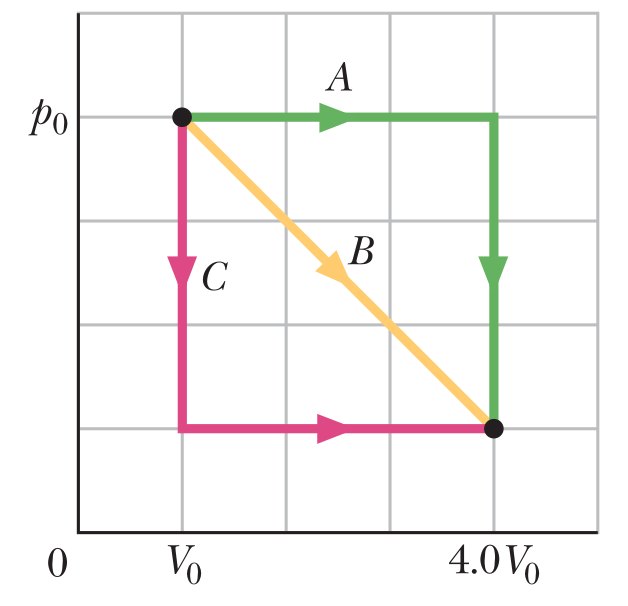
\includegraphics[width=0.75\textwidth]{Captura de tela de 2025-07-08 16-01-05.png}
                };
                \path (A.south west) -- (A.north west) node [midway, sloped] {Pressão (\si{Pa})};
                \path (A.south west) -- (A.south east) node [midway, yshift=-1ex] {Volume (\(\si{m^3}\))};
            \end{tikzpicture}
        \end{minipage}

    \item \ratio{33} Um bloco de cobre, de \(\SI{50}{g}\), cuja a temperatura é 
        \SI{117}{\celsius}, é colocado em uma caixa isolada junto com um bloco de chumbo de 
        \SI{100}{g} cuja temperatura é \SI{-80}{\celsius}. (a) Qual é a temperatura de equilíbrio
        do sistema de dois blocos? (b) Qual é a variação da energia interna do sistema 
        do estado inicial para o estado de equilíbrio? (c) Qual é a variação da 
        entropia do sistema?

    \item \ratio{34} Uma mistura de \SI{1773}{g} de água e \SI{327}{g} de gelo
        está inicialmente em equilíbrio a \SI{0}{\celsius}. A mistura é levada,
        por um processo reversível, a um segundo estado de equilíbrio no qual a 
        razão água-gelo, em massa, é 2:1 a \SI{0}{\celsius}. (a) Calcule a variação 
        de entropia do sistema durante esse processo. (b) O sistema é levado de volta
        ao estado de equilíbrio inicial por um processo irreversível (usando, por
        exemplo, um bico de Bunsen). Calcule a variação de entropia do sistema durante
        esse processo. (c) As respostas dos itens (a) e (b) são compatíveis com a 
        segunda lei da termodinâmica?

\end{enumerate}

Dados:
\begin{itemize}
    \item Calor específico do chumbo: \(\SI{128}{J/kg\cdot K}\)
    \item Calor específico do cobre: \(\SI{386}{J/kg\cdot K}\)
    \item Calor de fusão da água: \(\SI{333}{kJ/kg}\)
\end{itemize}

\newpage
\def\Description{Física Geral II -- Prova 3}

\begin{enumerate}
    \item%
        \begin{enumerate}
            \item Temos que 
                \[
                    W = W_\text{isobárico}+W_\text{isocórico} = 
                    p\Delta V + 0 =
                    3p_0V_0 =
                    \SI{225}{J}
                \]
            \item Temos que 
                \[
                    \begin{split}
                        W &= \int_{V_0}^{4V_0} p\;dV \\
                          &=\int_{V_0}^{4V_0}\left[\frac{p_0 - p_0/4}{V_0 - 4V_0}(V-V_0)+p_0\right]\;dV \\
                          &=\frac{p_0 - p_0/4}{V_0 - 4V_0}\frac{(4V_0-V_0)^2}{2}+p_0(4V_0 - V_0) \\
                          &=3p_0 V_0 - \frac{3V_0(p_0 - p_0/4)}{2}\\
                          &= \SI{140.625}{J}
                    \end{split}
                \]
            \item Temos que 
                \[
                    W = W_\text{isocórico}+W_\text{isobárico} = 
                    0 + p\Delta V=
                    3p_0V_0/4 =
                    \frac{\SI{225}{J}}{4} = \SI{56.25}{J}
                \]
        \end{enumerate}
    \item%
        \begin{enumerate}
            \item A temperatura de equilíbrio é dada por
                \[
                    T_f = \frac{m_\text{cobre}c_\text{cobre}T_\text{cobre} + m_\text{chumbo}c_\text{chumbo}T_\text{chumbo}}
                               {m_\text{cobre}c_\text{cobre} + m_\text{chumbo}c_\text{chumbo}}=
                               \SI{38.45}{\celsius}
               \]
           \item Como a caixa é isolada, não há energia saindo ou entrando no sistema e, portanto, a
               variação de energia interna é zero

           \item A variação de entropia é dada por
               \[
                   \Delta S = \Delta S_\text{cobre} + \Delta S_\text{chumbo} = 
                   m_\text{cobre}c_\text{cobre}\ln\frac{T_f}{T_\text{cobre}}+
                   m_\text{chumbo}c_\text{chumbo}\ln\frac{T_f}{T_\text{chumbo}}
               \]
                Mas, ao contrário do item (a), precisamos que as temperaturas estejam em kelvin
                \begin{align*}
                    T_\text{cobre} &= 117+273,15 = \SI{390.15}{K} \\
                    T_\text{chumbo} &= -80+273,15 = \SI{193.15}{K} \\
                    T_f &= 38,45+273,15=\SI{311.6}{K}
                \end{align*}
                Substituindo os valores, temos que \(\Delta S=\SI{1.78}{J/K}\)
        \end{enumerate}

    \item%
        \begin{enumerate}
            \item A massa total inicial é \(m_\text{tot} = \SI{1773}{g}+\SI{327}{g} = \SI{2100}{g}\) e, após o processo reversível,
                ela é dividida em 3 partes iguais de \(\SI{2100}{g}/3 = \SI{700}{g}\) onde 2 partes são de água (\SI{1400}{g}) e
                1 parte é de gelo (\SI{700}{g}). Dessa forma, podemos dizer que houve o congelamento de \(\SI{1773}{g}\SI{-1400}{g}=\SI{373}{g}\) de 
                água.

                Como o processo de congelamento ocorre a temperatura constante (processo isotérmico), temos que 
                \[
                    \Delta S = \frac{Q}{T} = -\frac{m L}{T} = -\frac{\num{373e-3}\cdot \num{333e3}}{273}=\SI{455}{J/K}
                \]
            \item Como a entropia é uma função de estado (não depende do processo), a variação de entropia é a mesma mas com
                o sinal trocado, já que estamos voltando ao estado inicial. Ou seja
                \[
                    \Delta S = \SI{-455}{J/K}
                \]

            \item Sim, as respostas são compatíveis com a segunda lei, pois em
                ambos os casos \(\Delta S_\text{universo} \geq 0\). 

                No item (a) a vizinhança remove calor do sistema de forma
                reversível, de forma que a variação de entropia do ''universo''
                é zero. Já no item (b), se o processo fosse reversível teríamos
                a variação de entropia do universo nula seguindo o mesmo
                raciocínio do item (a), mas como há irreversibilidades, há um
                ''extra'' de entropia sendo gerada e portanto a variação de
                entropia do universo é positiva.

                Os itens (a) e (b) não seriam compatíveis com a segunda lei
                somente se a variação de entropia do universo fosse negativa, o
                que só seria possível com uma ''fonte'' de entropia negativa, o
                que não existe.
        \end{enumerate}
       
\end{enumerate}
\end{document}
